\chapter{Introduction}
\label{chapter1}

\begin{bibunit}

\section{Fundamental Physics}

The discovery of the cosmic microwave background (CMB) radiation by \citet{1965ApJ...142..419P}
provided the first direct evidence that the universe had a beginning. Arno Penzias and Robert Wilson
shared the 1978 Nobel Prize in Physics for this discovery, and astronomers have been studying this
relic of the Big Bang ever since. In fact, a second Nobel Prize was awarded to John Mather and
George Smoot in 2006 for their work on the Cosmic Background Explorer (COBE) satellite, which was
amongst the first experiments to demonstrate that the background radiation was anisotropic
\citep{1992ApJ...396L...1S}. These studies of the CMB have fundamentally advanced humanity's
understanding of the universe: its origin, evolution, and composition. We continue to study the CMB
today in part because it illuminates everything in the universe. It is a flashlight for the darkness
of space within our expanding universe.

As the universe expands, the wavelength of a photon is similarly stretched or redshifted (so-called
because it gradually drifts to longer, redder wavelengths). Photons originating from a star 1000
light-year away will travel through the universe for 1000 years before they are collected by our
telescopes. Consequently, we observe this star as it was 1000 years ago. However, the photon was
also stretched by a small factor of $0.000007\%$ during its travels due to the expansion of the
universe.  For nearby stars, this expansion is too small to be conceivably measured.  However, with
the discovery of the first quasar by \citet{1963Natur.197.1040S} it soon became apparent that the
stretching factor, the redshift $z$, can be $>10\%$. Today, the most distant known quasars and
galaxies are so far away that the wavelength has more than doubled ($z > 1$) due to the expansion of
the universe \citep[e.g.,][]{2011Natur.474..616M, 2015ApJ...810L..12Z, 2016ApJ...819..129O,
2018Natur.553..473B}.

Due largely to careful and detailed work studying the CMB \citep[e.g.,][]{2013ApJS..208...19H,
2016A&A...594A..25P}, Type Ia supernova explosions \citep[e.g.,][]{1998AJ....116.1009R,
1999ApJ...517..565P}, and cosmological galaxy surveys \citep[e.g.,][]{2001MNRAS.328.1039C}, we have
a coherent and consistent understanding of the expansion history of the universe. The redshift $z$
is therefore commonly used as a proxy for distance. The higher the redshift, the longer the photon
has been in transit, and the further its origin. However, in order to measure the redshift, the
detected photon must originate from a known spectral feature.

Despite its abundance, neutral hydrogen (\ion{H}{1}) has few low energy transitions that allow it to
traced.  Due to this limitation, astronomers resort to using a hyperfine structure transition
arising from the magnetic dipole interaction between proton and electron. This interaction leads to
a slight energy difference between the spin-symmetric state and the spin-antisymmetric state. The
energy difference is $hc / (21\,\text{cm})$ where $h$ is Planck's constant, and $c$ is the speed of
light.  When a hydrogen atom transitions from the spin-symmetric state (higher energy; $F=1$) to the
spin-antisymmetric state (lower energy; $F=0$), it emits a photon with a wavelength of
$21\,\text{cm}$ or a frequency of $1420\,\text{MHz}$. The redshift $z$ of a 21\,cm photon is
therefore computed from the observed frequency $\nu$ as
\begin{equation}\label{eq:redshift-equation}
    z = \frac{1420\,\text{MHz}}{\nu} - 1\,.
\end{equation}
The 21\,cm transition is exceptionally weak.  The half-life of a neutral hydrogen atom in the $F=1$
state is over 10\,Myr.  However, the early universe following recombination is almost entirely
composed of neutral hydrogen.

When \ion{H}{1} is illuminated by the CMB, a portion of the incident photons are 21\,cm photons.
These photons can be absorbed by a hydrogen atom in the $F=0$ state, or stimulate the emission of
21\,cm photon from a hydrogen atom in the $F=1$ state.  A careful calculation of the radiative
transfer for a clump of atomic hydrogen gas illuminated by the CMB at the redshift $z$ yields
\citep[][but neglecting the contribution of peculiar velocities]{2012RPPh...75h6901P}
\begin{equation}\label{eq:radiative-transfer-equation}
    \Delta T_{21} \approx 27 \left[
        \overbrace{
            x_\text{HI} (1+\delta)
            \left(\frac{\Omega_b h}{0.0327}\right)
        }^{\text{quantity of HI}}
        \left(\frac{\Omega_m}{0.307}\right)^{-1/2}
        \left(\frac{1+z}{10}\right)^{1/2}
        \overbrace{
            \left(\frac{T_\text{spin} - T_\text{CMB}(z)}{T_\text{spin}}\right)
        }^{\text{relative temperature}}
    \right] \, {\rm mK} \,,
\end{equation}
where $\Delta T_{21}$ is the expected 21\,cm brightness temperature. If $\Delta T_{21} > 0$, the
21\,cm transition appears in emission against the CMB. If $\Delta T_{21} < 0$, it appears in
absorption. $x_\text{HI}$ is the neutral fraction of hydrogen, $\delta$ is the local baryon
overdensity, $h$ is the Hubble constant, $\Omega_b$ is the density parameter for baryons, $\Omega_m$
is the density parameter for matter, $T_\text{spin}$ is the spin temperature (the excitation
temperature of the 21\,cm transition), and $T_\text{CMB}(z) = 2.73\,(1+z)\,{\rm K}$ is the
temperature of the CMB at the redshift $z$.

\begin{figure}[t]
    \centering
    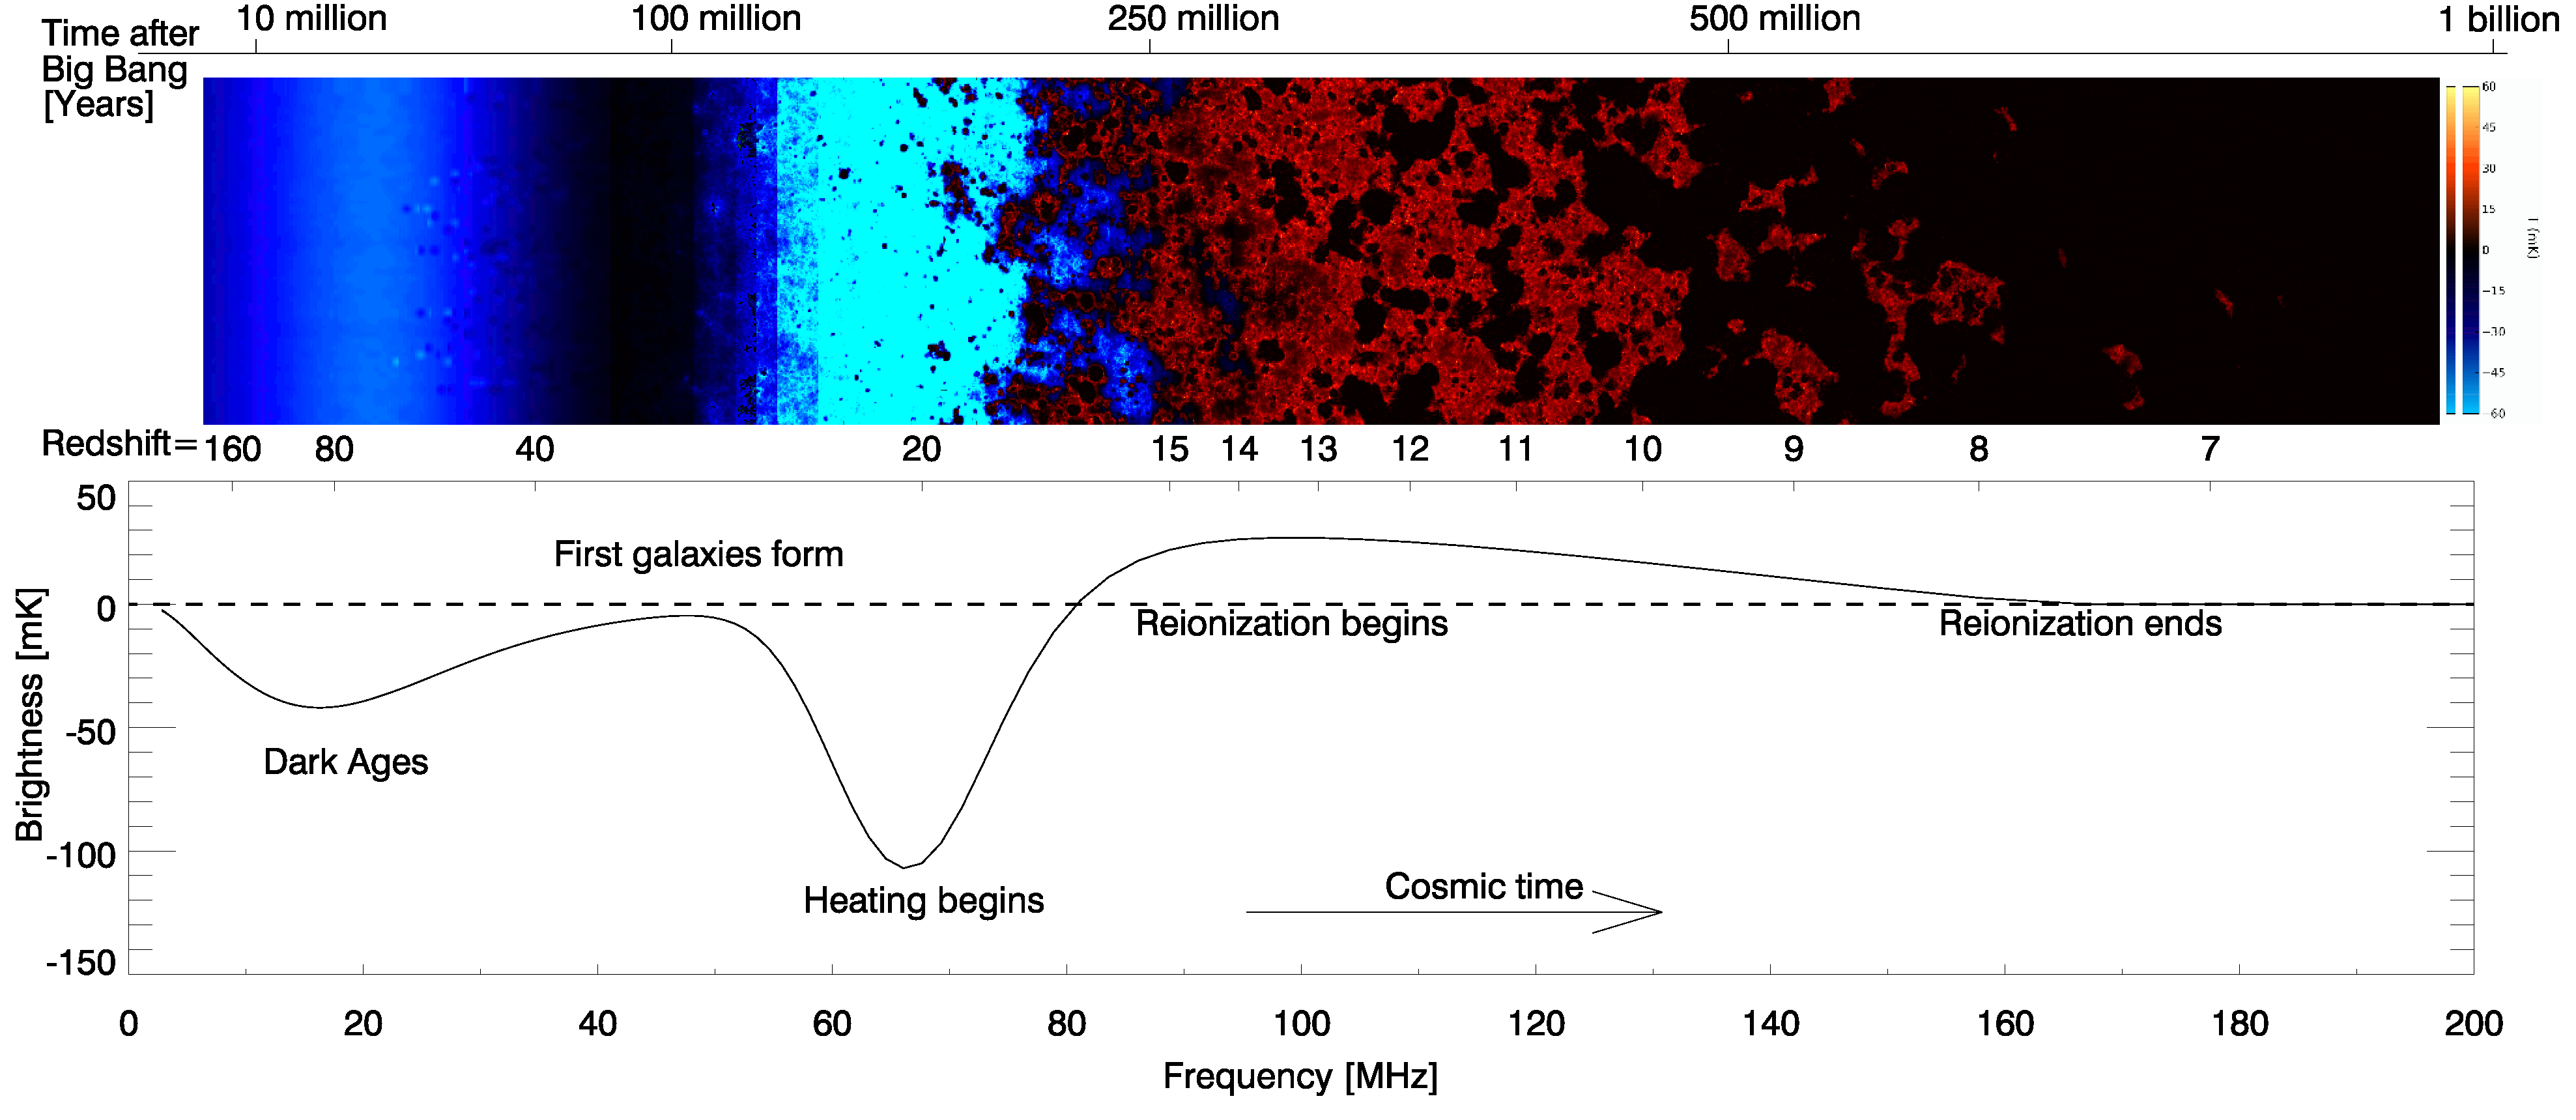
\includegraphics[width=\textwidth]{figures/chapter1/pritchard-2012-global-signal}
    \caption{
        (top) A simulated light cone of the 21\,cm brightness temperature illustrating the
        anisotropy in the expected signal.
        (bottom) A simulation of the globally averaged brightness temperature due to the high
        redshift 2\,~cm transition.
        This figure is reproduced with permission from \citet{2012RPPh...75h6901P}.
    }
    \label{fig:pritchard-global-signal}
\end{figure}

Equation~\ref{eq:radiative-transfer-equation} is fundamental to determining what can be learned
through detecting the 21\,cm transition at high redshift. First, the 21\,cm transition of neutral
hydrogen at $z\sim 10$ can perturb the 2.73\,K thermal CMB spectrum by typically 10--100\,mK.
Second, If the spin temperature is greater than the CMB temperature, the 21\,cm transition appears
in emission. However, the signal saturates at high spin temperatures. If the spin temperature is
less than the CMB temperature, the 21\,cm transition appears in absorption with no saturation point.
There is no measurable 21\,cm signal if the transition is in radiative equilibrium with the CMB.
Finally, the amplitude of the signal is proportional to the total quantity of \ion{H}{1}. Therefore,
the amplitude tends to be larger while the universe is predominantly neutral.  Because redshift can
be computed from the observed frequency (Equation~\ref{eq:redshift-equation}), the highly redshifted
21\,cm transition can be used to map the three dimensional structure of the universe and chronicle
its history through the Cosmic Dawn and Epoch of Reionization (EoR).  A fiducial prediction for
$\Delta T_{21}(z)$ can be seen in Figure~\ref{fig:pritchard-global-signal}.

\section{A History of the Universe through the 21\,cm Transition}

There are three relevant temperatures that affect the spin temperature: $T_\text{gas}$, the
temperature of the gas, $T_\text{CMB}$, the temperature of the CMB, and $T_{\text{Ly}\alpha}$, the
color temperature of the Ly$\alpha$ radiation from early star formation. More exotic theories might
also include the temperature of the dark matter, $T_\text{DM}$. Generally, Ly$\alpha$ photons
scatter through the intergalactic medium (IGM), which sets $T_{\text{Ly}\alpha} = T_\text{gas}$. In
the absence of any heating mechanisms, the matter and radiation are both cooling adiabatically with
the expansion of the universe.  The adiabatic indices are $\gamma = 5/3$ and $\gamma = 4/3$
respectively, so the matter cools faster than the radiation. Consequently, the 21\,cm transition
tends to appear in absorption prior to early star formation, and in emission after the IGM has been
heated.

While there are currently few observational constraints on the 21\,cm brightness temperature,
fiducial theoretical models tell the following story \citep[e.g.,][]{2006PhR...433..181F,
2012RPPh...75h6901P}.  Prior to star formation---the dark ages ($z \gtrsim 40$)---the density of the
universe is high enough for collisions between hydrogen atoms to dominate the excitation of the
21\,cm transition.  During this time $T_\text{spin} = T_\text{gas}$, and the 21\,cm transition
appears in absorption against the CMB.  Later ($z \sim 30$), as the mean density of the universe
decreases, collisions become more infrequent and the 21\,cm transition is instead excited by CMB
photons. During this time the 21\,cm signal vanishes because $T_\text{spin} = T_\text{CMB}$.

With the onset of star formation in the universe, the Cosmic Dawn, the IGM is inundated with
Ly$\alpha$ photons.  These Ly$\alpha$ photons scatter through the IGM. With the absorption and
re-emission of a Ly$\alpha$ photon, a hydrogen atom can transition between the spin-symmetric state
and the spin-antisymmetric state. This process, called the Wouthuysen-Field effect, sets the
relative abundance of \ion{H}{1} in each state such that $T_\text{spin} = T_{\text{Ly}\alpha} =
T_\text{gas}$ \citep{1952AJ.....57R..31W,1958PIRE...46..240F}. Therefore, after early star formation
begins, the 21\,cm transition reappears in absorption against the CMB.

However, as star formation progresses, the gas in the IGM is heated. X-rays are particularly
effective at heating the IGM due to their large mean-free path. Consequently the heating rate is
sensitive to, for example, the number density, luminosity and spectral hardness of X-ray binaries
\citep{2014MNRAS.437L..36F,2017MNRAS.472.2651G}.  Eventually the gas is heated above the temperature
of the CMB, bringing the 21\,cm transition into emission, and eventually the signal saturates. At
this point the 21\,cm transition begins to disappear with the onset of reionization at $z \lesssim
15$ due to the ionization of the IGM. A prediction of the spectral distortion this process applies
to the low-frequency ($\nu < 200\,\text{MHz}$) CMB spectrum can be seen in the bottom panel of
Figure~\ref{fig:pritchard-global-signal}.

Due to the extremely wide fields of view of low-frequency radio telescopes, the use of the 21\,cm
transition is unique in its ability to directly probe the temperature, density, and ionization state
of the IGM over extremely large volumes. However, the EoR is also the focus of a number of other
complementary studies that inform this prediction. Careful observations of the CMB constrain the
mean redshift of reionization through the Thomson scattering optical depth, and the duration of
reionization through the kinetic Sunyaev--Zel'dovich (kSZ) effect. The final nine-year results from
the Wilkinson Microwave Anisotropy Probe (WMAP) favored a mean reionization redshift of $z\sim10$
\citep{2013ApJS..208...19H}. More recently, the Planck experiment measured a lower optical depth
that prefers a reionization history with a mean at $z\sim7.8-8.8$ and a duration of $\Delta z < 2.8$
\citep{2016A&A...596A.108P}, which is easier to reconcile with the measured ultraviolet (UV)
luminosity functions of high-redshift galaxies.

The discovery of ever-distant high-redshift galaxies has begun to constrain the ultraviolet
luminosity function during the EoR. These galaxies are typically discovered by searching for the
Lyman break in deep galaxy surveys \citep[pioneered by][]{1996ApJ...462L..17S}.  The most distant
spectroscopically confirmed galaxy is GN-z11 at $z\approx 11.1$ \citep{2016ApJ...819..129O}. An
image of this galaxy can be seen in Figure~\ref{fig:oesch-galaxy}.  The UV luminosity function
constrains the number of ionizing photons generated by these high-redshift galaxies, however
flux-limited galaxy surveys necessarily only discover the most exceptionally luminous galaxies. In
contrast, measuring the 21\,cm brightness temperature will constrain the integrated UV luminosity
function.  Current limits (including a ``reasonable'' extrapolation to unseen fainter galaxies)
suggest that high-redshift star-forming galaxies produce enough photons to ionize the universe on a
timescale consistent with constraints from the CMB \citep{2015ApJ...802L..19R}.

\begin{figure}[t]
    \centering
    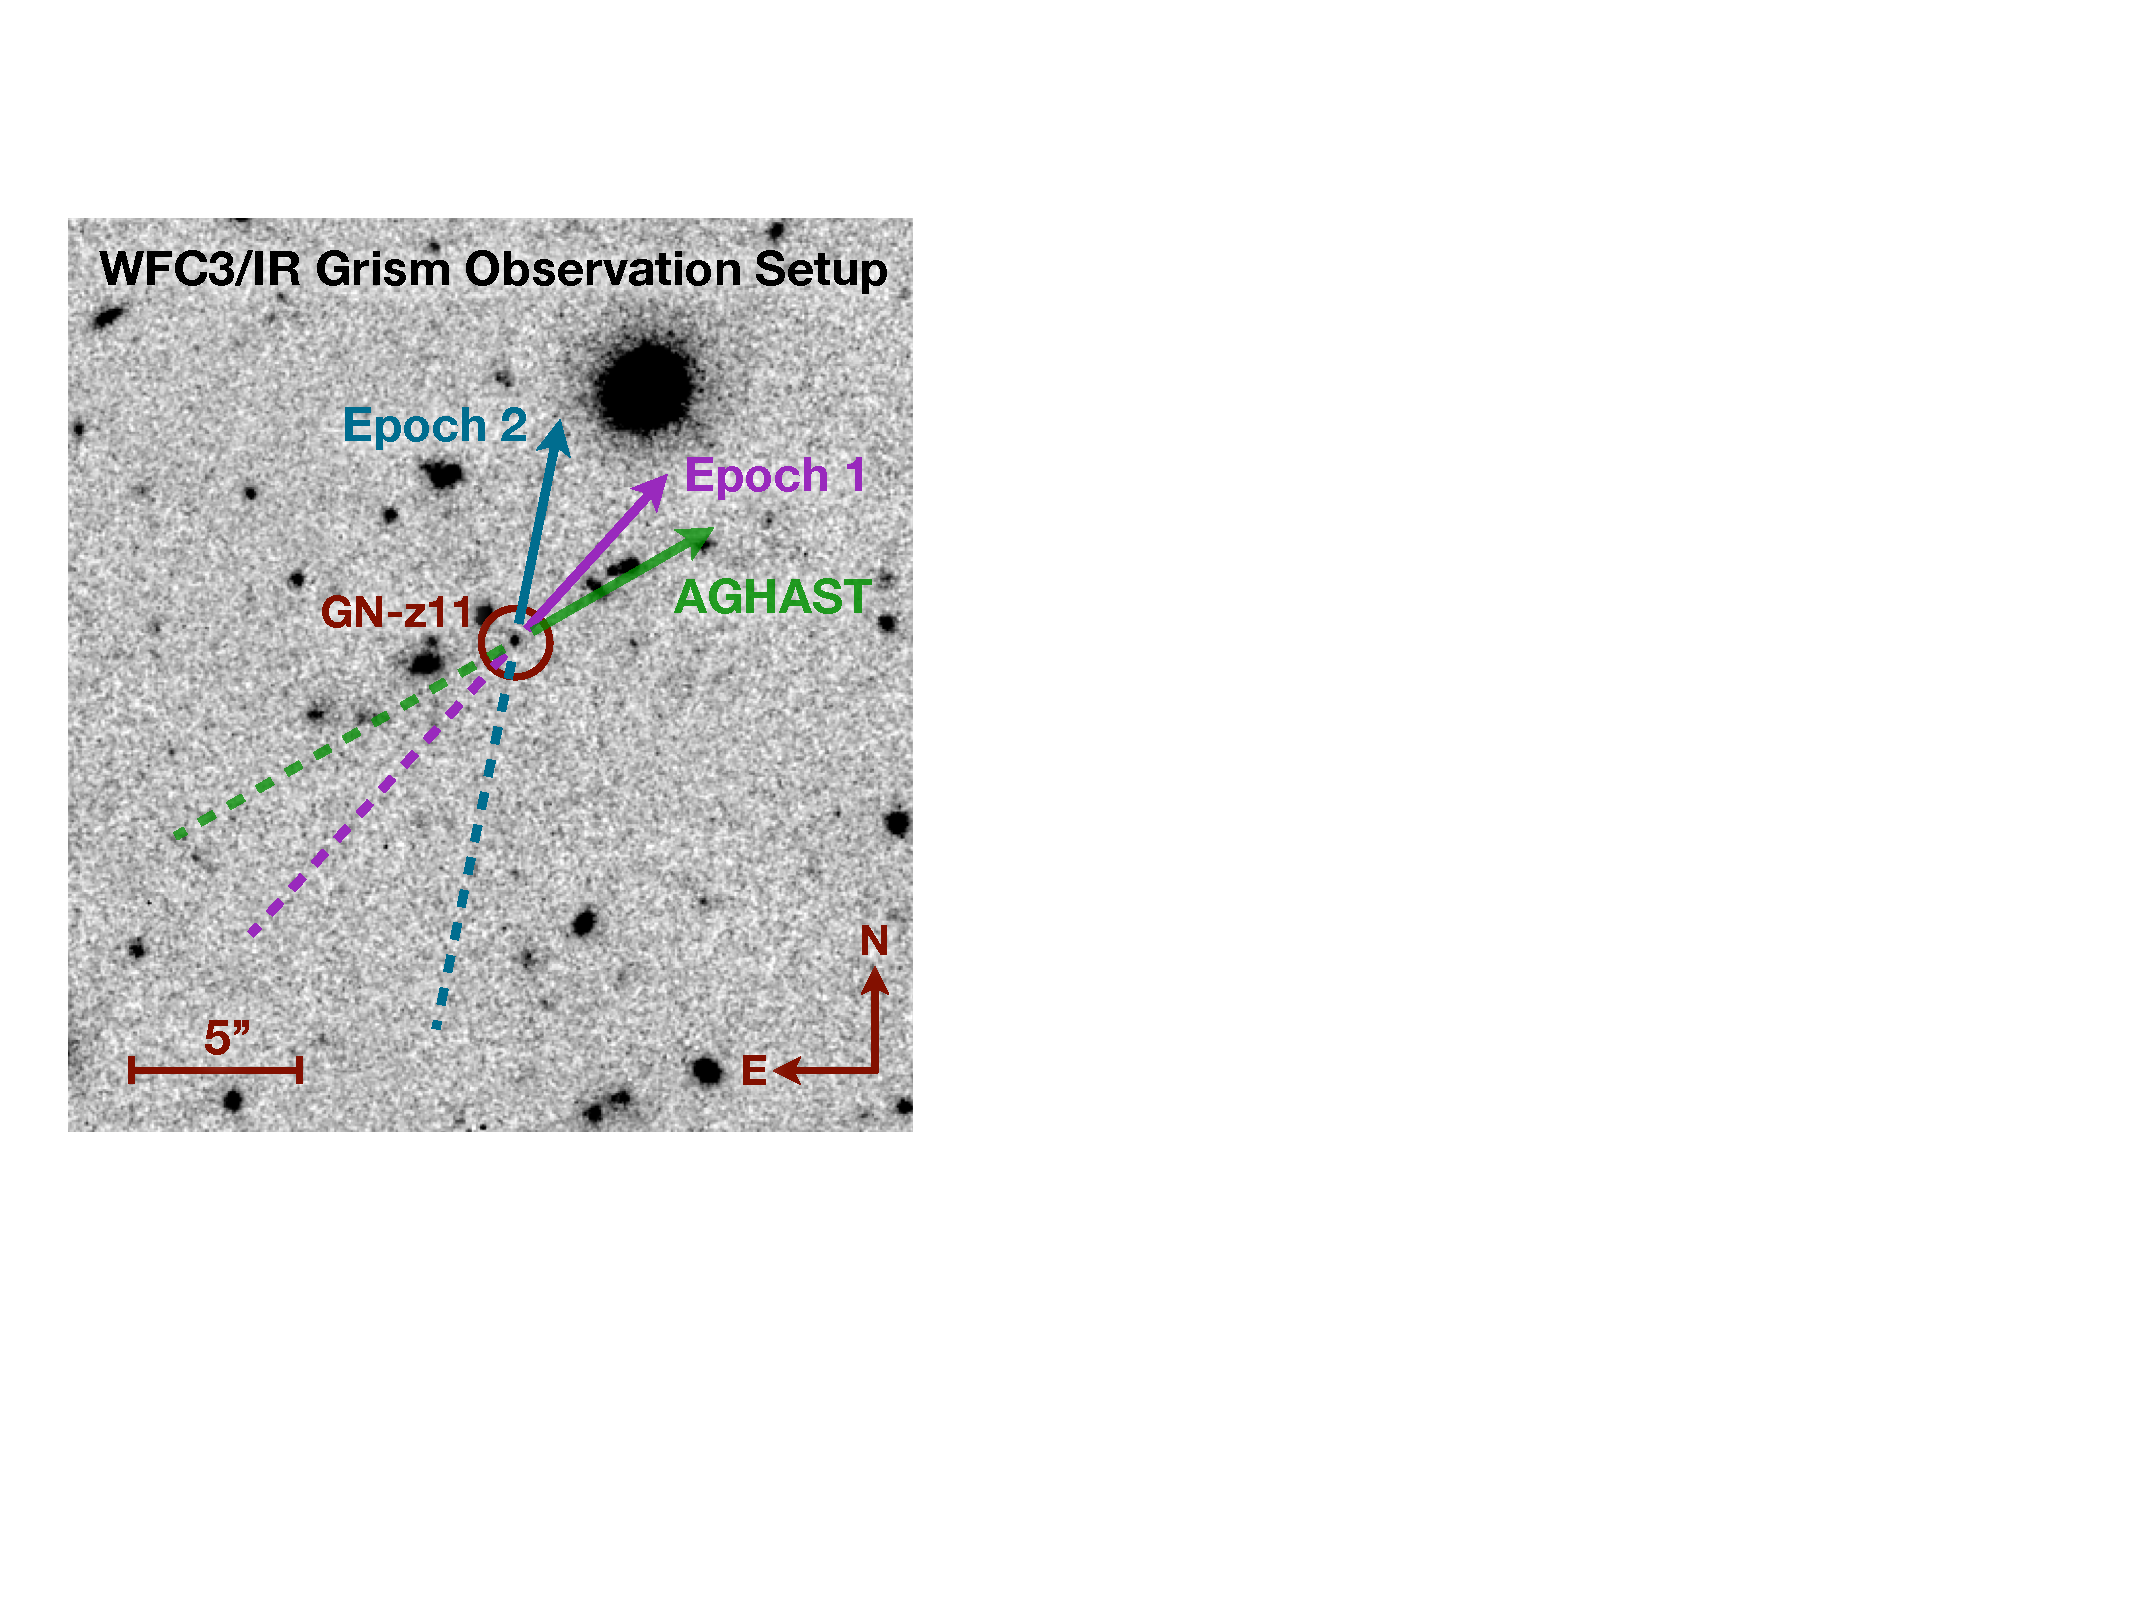
\includegraphics[width=\textwidth]{figures/chapter1/oesch-gn-z11}
    \caption{
        An $H$-band image of GN-z11, the most distant spectroscopically confirmed galaxy with the
        dispersion direction for the Hubble Space Telescope grism spectra that confirmed that this
        galaxy originates from $z\approx11.1$. This figure is reproduced from
        \citet{2016ApJ...819..129O}. \textbf{get permission to republish this figure}
    }
    \label{fig:oesch-galaxy}
\end{figure}

The timing of reionization has also been constrained by the discovery of high-redshift quasars,
which can be used to map the Ly$\alpha$ opacity---and hence the neutral fraction of hydrogen---along
the line of sight.  Variations between lines of sight additionally provides evidence for the
patchiness of reionization (see Figure~\ref{fig:fan-quasars}). The highest redshift quasars at
$z>7$, however, are exceptionally rare.  \citet{2011Natur.474..616M} discovered a quasar at
$z\approx7.1$, and by measuring the damping wing of the near-zone Ly$\alpha$ absorption determined
that the neutral fraction is at least 0.1 in the vicinity of this quasar.
\citet{2018Natur.553..473B} found another quasar at $z\approx7.5$ and performed a similar analysis
to determine that the neutral fraction is at least 0.33. The EoR therefore appears to be in progress
and drawing to a close by $z\sim 6$.

\begin{figure}[p]
    \centering
    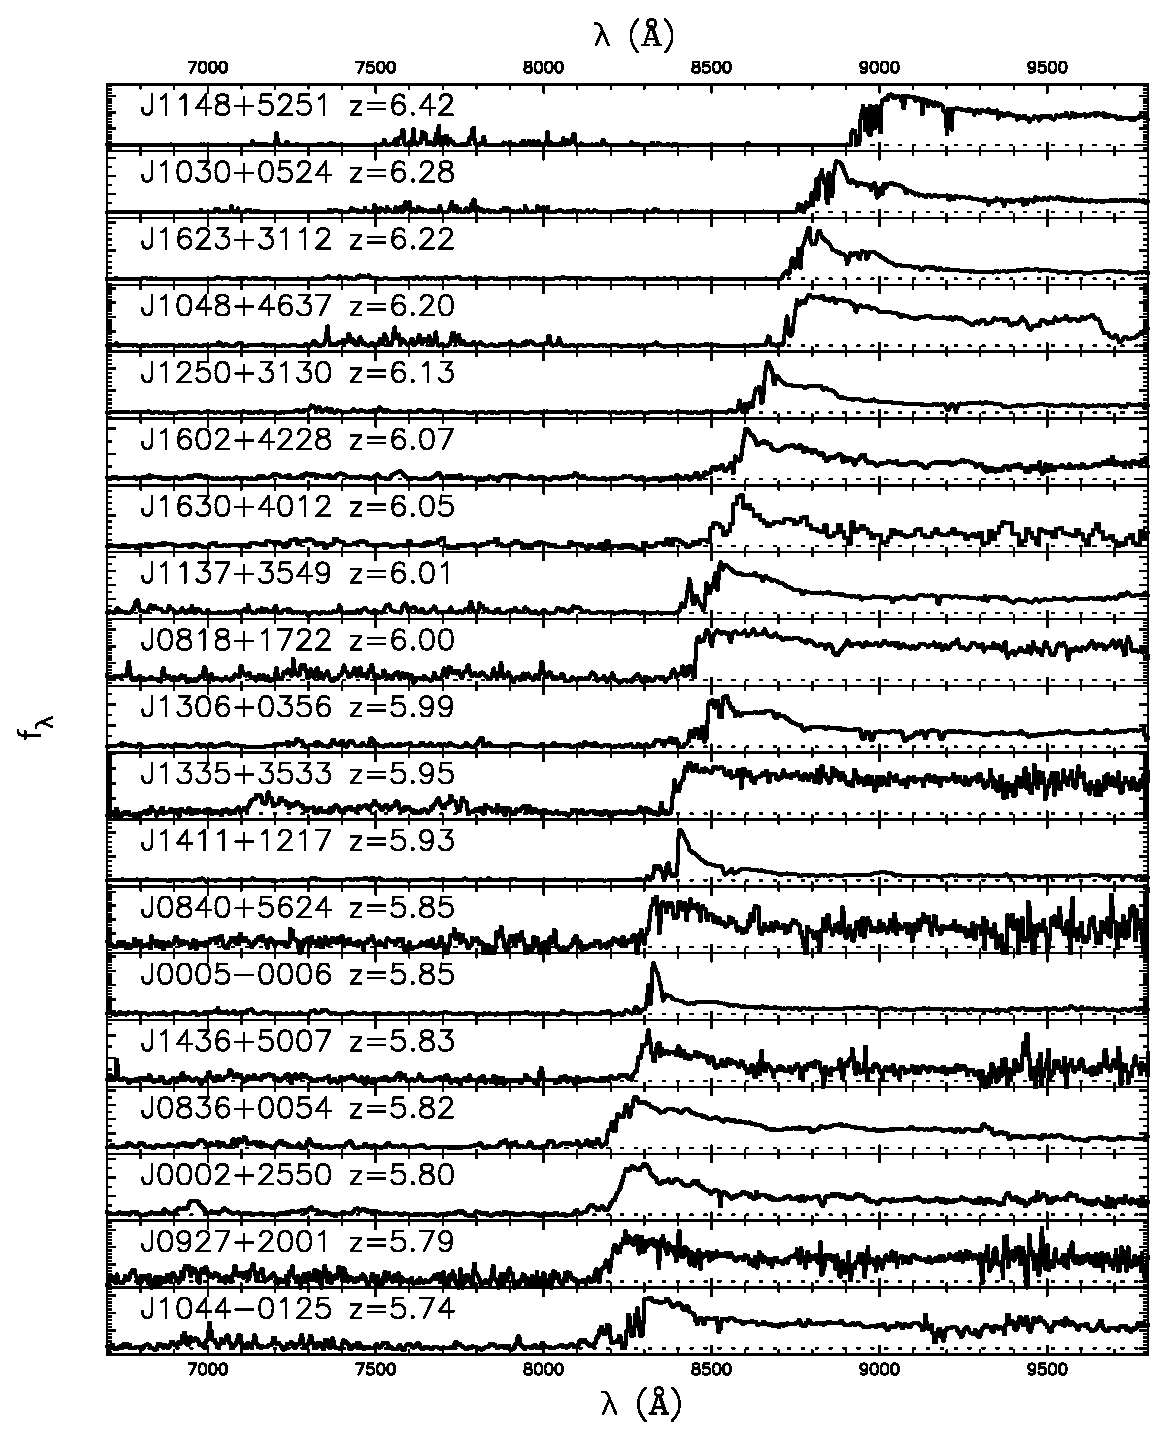
\includegraphics[width=\textwidth]{figures/chapter1/fan-quasar-spectra}
    \caption{
        A collection of spectra for high-redshift quasars illustrating the trend towards a
        completely saturated Gunn--Peterson trough with increasing redshift, but variations between
        quasars at comparable redshifts provide evidence for patchy reionization. This figure is
        reproduced from \citet{2006AJ....132..117F}. \textbf{get permission to republish this
        figure}
    }
    \label{fig:fan-quasars}
\end{figure}

\section{First Generation 21\,cm Experiments}

The first successful attempt make use of the 21\,cm emission to map the three-dimensional structure
of the universe was conducted by \citet{2010Natur.466..463C} using the Green Bank Telescope (GBT)
across redshifts 0.53--1.12. This measurement demonstrated the feasibility of using low-resolution
spectral-line maps to study Baryon Acoustic Oscillations (BAO) at the onset of the accelerating
expansion of the universe.

Ultimately, it may be possible to map the EoR and Cosmic Dawn through the 21\,cm line
\citep{1997ApJ...475..429M}. In fact, this is called a ``main science goal'' for the future Square
Kilometer Array \citep[SKA;][]{2013ExA....36..235M}.  First generation experiments, however, are of
somewhat more limited scope and therefore employ statistical averages to boost sensitivity to the
high-redshift 21\,cm signal.

The two most popular statistics are the global average and the power spectrum. The global
average---or monopole---is computed by averaging over all lines of sight. The global signal is
therefore simply the mean 21\,cm brightness temperature within a spherical shell of the universe:
\begin{equation}
    T^\text{global}_{21}(z) = \frac{1}{\Omega}\int \Delta T_{21}(z; \hat{r}) \, \d\Omega \,,
\end{equation}
where $T^\text{global}_{21}(z)$ is the global 21\,cm signal at the redshift $z$, $\Delta
T_{21}(z; \hat{r})$ is the 21\,cm brightness temperature at the redshift $z$ in the direction
$\hat{r}$, and the integral runs over solid angle $\Omega$.

The power spectrum statistic leverages the line of sight distance information from the observed
frequency to measure the power in fluctuations on a given spatial scale within a volume of the
universe:
\begin{equation}
    P_{21}(z; \vec{k}) =
        \frac{1}{V}\left|
        \int \Delta T_{21}(\vec{r}) \, e^{-i\vec{k}\cdot\vec{r}} \, \d^3r
        \right|^2\,,
\end{equation}
where $P_{21}(z; \vec{k})$ is the three-dimensional spatial power spectrum at the redshift $z$ and
wavevector $\vec{k})$, and the integral runs over the observed volume $V$ of the universe.
Neglecting redshift-space distortions, the spatial power spectrum of 21\,cm fluctuations is expected
to be isotropic. Therefore, typically the power spectrum $P(\vec{k})$ is averaged over the
orientation of the wavevector $\vec{k}$. Instrumental considerations typically lead to different
sources of systematic errors along the line of sight and perpendicular to the line of sight, so
parameterizing the power spectrum in terms of the parallel and perpendicular to the line of sight
wavenumbers ($k_\parallel$ and $k_\perp$ respectively) is common.

The global signal and the power spectrum are both statistics of the same underlying 21\,cm
brightness temperature and therefore both statistics can be used to answer high-level questions such
as: When did reionization occur? How quickly was the universe heated after initial star formation
began?  The power spectrum contains additional information about the sources of heating and
ionization.  During the Cosmic Dawn, a detection of the 21\,cm power spectrum could constrain the
X-ray emissivity and spectral hardness \citep{2014MNRAS.437L..36F} the strength of Lyman--Werner
feedback \citep{2013MNRAS.432.2909F}, and the spatial scale on which this X-ray emission originates.
During the EoR, a detection of the 21\,cm power spectrum could constrain the ionizing efficiency of
early galaxies, the mean-free path of ionizing photons, and the minimum halo mass for star formation
\citep{2015MNRAS.449.4246G}.  However, both approaches are complementary because they employ
substantially different instrumental designs and are subject to different (but not exclusively
different) systematic errors.

\subsection{Global Signal Experiments}

Most global signal experiments are composed of a single dipole antenna with a total power
radiometer. This approach was pioneered by the Experiment to Detect the Global EoR Signature
(EDGES). After deploying to the Murchison Radio-astronomy Observatory (MRO) in a remote region of
Western Australia, \citet{2010Natur.468..796B} observed for three months. If reionization was an
instantaneous event, this initial EDGES deployment would have expected to see a step function in
their sky-averaged spectrum. Therefore the authors converted the observed spectral smoothness to a
lower bound on the duration of reionization $\Delta z > 0.06$. However, because no such feature was
detected, the redshift of reionization was not constrained by this measurement.

EDGES has continued to improve on this initial constraint.  \citet{2017ApJ...847...64M} reported
results from the updated EDGES high-band instrument (90--190\,MHz), which now rules out most
reionization histories with $\Delta z \lesssim 0.4$ and histories with $\Delta z \lesssim 1.0$ if
the central redshift of reionization is near $z\approx 8.5$. Even more recently,
\citet{2018Natur.555...67B} reported results from the new EDGES low-band instrument (50--100\,MHz),
which is effectively a scaled copy of the high-band instrument. The latter results will be discussed
in more detail in \S\ref{sec:intro-future-outlook}.

The Large-aperture Experiment to Detect the Dark Age \citep[LEDA;][]{2018MNRAS.478.4193P} similarly
equips low-frequency (30--85\,MHz) dipole antennas with radiometers. Located at the Owens Valley
Radio Observatory (OVRO) near Big Pine, California, these antennas are embedded within the OVRO-LWA.
This configuration provides LEDA with additional leverage for self-calibration and foreground
imaging, which may prove crucial for overcoming latent concerns about beam modeling and foreground
removal in many global signal experiments.

The SARAS~2 experiment, like EDGES, is a single antenna radiometer. However, SARAS~2 has chosen an
unconventional sphere-disk monopole antenna in order to minimize the frequency structure in the
antenna response pattern. \citet{2017ApJ...845L..12S} reported initial results from a 63~hr
integration over the frequency range 110--200\,MHz from the Timbaktu Collective in Southern India.
By comparing against parameterized models of the 21\,cm signal, the authors concluded that their
initial results generally rule out models with weak X-ray heating and rapid reionization. These
models generally produce sharp spectral features in the observing band, and so this limit arises
from the measured spectral smoothness.

Although most global signal experiments are composed of isolated dipole antennas, there have been
several attempts to design and use more exotic instruments. \citet{2013PhRvD..87d3002L} found that
an instrument with a 5$\arcdeg$ beam could achieve a higher significance detection by using the
improved angular resolution to mitigate foreground contamination. \citet{2015MNRAS.450.2291V} used
lunar occultation to constrain the global signal between 35 and 80\,MHz using LOFAR. This technique
uses an interferometer to measure the contrast between the moon and the surrounding sky, but is
complicated by radio frequency interference (RFI) reflecting off of the moon and potentially by the
assumption that the moon is a thermal source at low frequencies. Drawn by the calibration advantages
of interferometers, other groups have proposed designing interferometers that have nonzero
sensitivity to the monopole. \citet{2015ApJ...809...18P} developed a framework for measuring the
global signal from interferometric measurements, and \citet{2015ApJ...815...88S} designed a
zero-spacing interferometer using a resistive screen to separate two antennas. However, ultimately
the calibration advantages of using an interferometer to measure the global signal may have been
overstated.  \citet{2016ApJ...826..116V} demonstrated that interferometers may only have any
sensitivity to the global signal if there is some amount of cross talk between the correlated
elements or a source of noise that can radiate coherently into both receivers.

\subsection{Power Spectrum Experiments}

\begin{figure}[t]
    \centering
    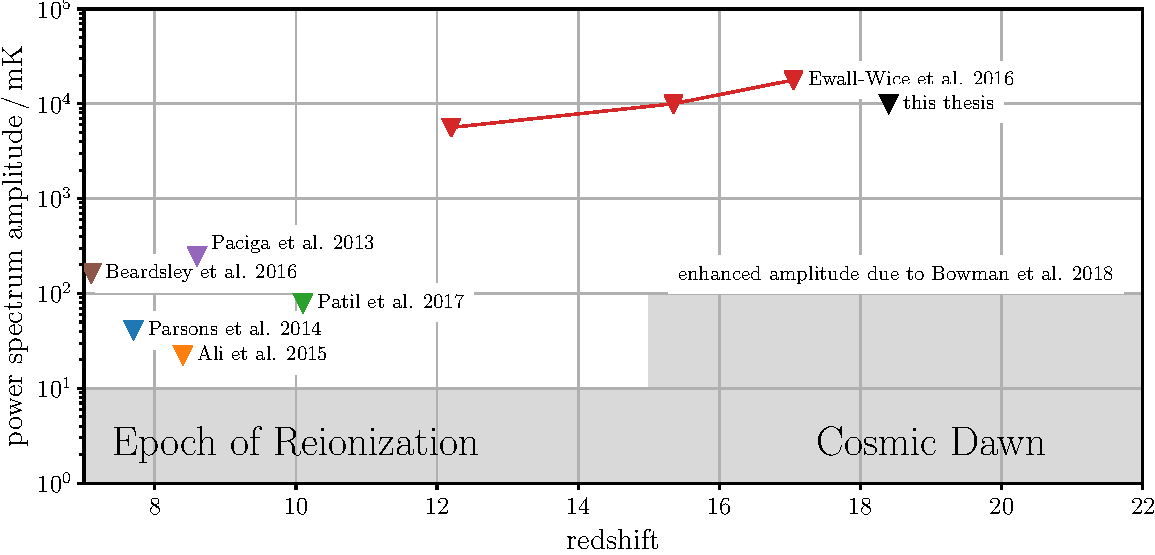
\includegraphics[width=\textwidth]{figures/chapter1/power-spectrum-upper-limits/power-spectrum-upper-limits}
    \caption{
        Power spectrum amplitude upper limits (95\% confidence or lowest systematically limited data
        point) as a function of redshift. The shaded region denotes roughly where current
        theoretical predictions fall.
    }
    \label{fig:power-spectrum-upper-limits}
\end{figure}

In contrast to the global signal experiments, which are typically composed of a single antenna,
power spectrum experiments are generally interferometers composed of up to hundreds or thousands of
antennas. A high-level overview of existing upper limits on the 21\,cm power spectrum can be seen in
Figure~\ref{fig:power-spectrum-upper-limits}.

The Donald C. Backer Precision Array for Probing the Epoch of Reionization
\citep[PAPER;][]{2010AJ....139.1468P} began attempting to measure the 21\,cm power spectrum with a
deployment of eight antennas in Green Bank, West Virginia. Later deployed with 32 antennas to the
Karoo desert in South Africa, \citet{2014ApJ...788..106P} measured a $2\sigma$ upper limit of
$(41\,\text{mK})^2$ on the amplitude of the power spectrum at $z=7.7$. This measurement ruled out
the possibility that the universe was entirely unheated by this redshift.  Later, with PAPER now
composed of 64 antennas, \citet{2015ApJ...809...61A} improved the best $2\sigma$ upper limit to
$(22.4\,\text{mK})^2$ at $z=8.4$, however this result is currently subject to revision due to a
number of errors including unexpected signal loss and underestimated error bars (Cheng et al. in
prep.). PAPER is notable for its decision to part with traditional interferometry. Starting with its
32-antenna deployment, PAPER opted for a maximally redundant antenna configuration, which maximizes
the interferometer's raw sensitivity to a particular spatial scale.

The Low-Frequency Array (LOFAR) EoR Key Science Project (KSP) is attempting a similar measurement of
the 21\,cm power spectrum. In contrast to PAPER, LOFAR is composed of $\sim30,000$ high-band
antennas (120--240\,MHz) and $\sim3,000$ low-band antennas (30--80\,MHz). These antennas are grouped
into stations and stations are correlated with each other. This design is a trade off that
sacrifices field of view for gain. The LOFAR EoR KSP recently published its first limits on the
21\,cm power spectrum, finding a $2\sigma$ upper limit of $(79.6\,\text{mK})^2$ at $z=10.1$
\citep{2017ApJ...838...65P}. In this measurement, LOFAR attempted to leverage its superior imaging
and source-removal capabilities, but ultimately this measurement was limited by residual systematic
errors. The removal of contaminating diffuse radio emission has been the focus of ongoing work with
some reported success \citep{koopmans_2017}.

Several attempts have been made to measure the 21\,cm power spectrum with the Murchison Widefield
Array (MWA) using multiple different techniques \citep{2016ApJ...825..114J}.
\citet{2016ApJ...833..102B} reported results from the first season of observing, and placed an upper
limit of $(164\,\text{mK})^2$ at $z=7.1$ with a 32\,hr integration.  While all previous power
spectrum measurements had attempted to constrain the power spectrum of 21\,cm fluctuations during
the EoR, \citet{2016MNRAS.460.4320E} used the MWA to place upper limits on the 21\,cm power spectrum
during the Cosmic Dawn.  In their highest redshift measurement, the authors placed a limit of $\sim
(18,000\,\text{mK})^2$ at $z\sim 17$. A simple comparison between these two upper limits from the
MWA illustrates the difficulty involved with constraining the Cosmic Dawn at a higher redshift than
the EoR.

Finally, the Giant Metrewave Radio Telescope (GMRT) EoR experiment, located near Pune, India, first
reported a $2\sigma$ upper limit of $(70\,\text{mK})^2$ at $z \approx 8.6$
\citep{2011MNRAS.413.1174P}.  However, this limit was later revised to $(248\,\text{mK})^2$ after a
careful study of the signal loss associated with foreground removal \citep{2013MNRAS.433..639P}.

\section{Observational Challenges}

The two most substantial challenges faced by all attempts to measure the cosmological 21\,cm
emission are:
\begin{enumerate}
    \item
        the blindingly bright foreground radio emission that must be subtracted, removed, or
        otherwise suppressed, and
    \item
        the instrumental calibration, which must be completed with a high degree of accuracy or else
        residual foreground emission could be confused with the cosmological 21\,cm signal.
\end{enumerate}

\subsection{Foreground Emission}

Prior to the commencement of this thesis, the most commonly used model of the low-frequency sky was
the Global Sky Model \citep[GSM;][]{2008MNRAS.388..247D}. The GSM is effectively an interpolation of
previously published sky maps between 10\,MHz and 100\,GHz. However, the majority of the modern,
high fidelity sky maps are located at frequencies above 1.4\,GHz. Below 1.4\,GHz, there is the
408\,MHz Haslam map \citep{1981A&A...100..209H,1982A&AS...47....1H}, which covers the sky at
1$\arcdeg$ resolution. At 45\,MHz, \citet{2011A&A...525A.138G} compiled a sky map from a northern
hemisphere survey and a southern hemisphere survey each at 5$\arcdeg$ resolution
\citep{1997A&AS..124..315A, 1999A&AS..140..145M}. At 22\,MHz, \citet{1999A&AS..137....7R} mapped the
sky from the Canadian Dominion Radio Astrophysical Observatory (DRAO) at 1$\arcdeg$--2$\arcdeg$
resolution.

At large angular scales $\theta \gg 1\arcdeg$, the low-frequency radio sky is dominated by galactic
synchrotron emission generated by relativistic electrons spiraling around galactic magnetic field
lines. The EDGES experiment, in the southern hemisphere, measured the brightness temperature of this
emission at \emph{high} galactic latitudes to be \citep{2017MNRAS.464.4995M}
\begin{equation}\label{eq:edges-sky-spectrum}
    T \sim 300\,\left(\frac{\nu}{150\,{\rm MHz}}\right)^{-2.6}\,\text{K}.
\end{equation}
At smaller angular scales $\theta \ll 1\arcdeg$, the galactic emission gives way to a sea of active
galactic nuclei (AGN), the brightest of which---Cyg A---has a flux $>15,000\,\text{Jy}$ at frequencies
$<80\,\text{MHz}$ \citep{1977A&A....61...99B}. A simple comparison between
Equations~\ref{eq:radiative-transfer-equation} and \ref{eq:edges-sky-spectrum} reveals that the
foreground radio emission must be suppressed by four to five orders of magnitude before the 21\,cm
fluctuations can be detected.  However, this foreground emission is typically synchrotron and
free-free, both of which generate smooth power-law spectra. The 21\,cm signal, on the other hand, is
not expected to be so smooth. This is due to the fact that sweeping through frequency along a line
of sight probes different causally disconnected regions of the universe. Each of these regions
experiences a different star formation, heating and reionization history, which ultimately produces
a different 21\,cm brightness temperature.  While spectral structure can be used to separate the
signal from contaminating foreground emission, there is still a relative paucity of suitable modern,
high-fidelity sky maps at frequencies $<200\,\text{MHz}$.

Compounding the problem, global signal experiments have no intrinsic angular resolution of their
own. To date, these experiments have typically relied on low-order polynomial fits to remove the
foreground contamination in their measurements. This is a fine balancing routine, because if the
polynomial order is chosen to be too low, residual foreground contamination dominates the
measurement. If the polynomial order is chosen to be too high, the 21\,cm signal itself can be
removed. Similarly, some power spectrum experiments, notably PAPER, have opted for a maximally
redundant baseline configuration that greatly inhibits the interferometer's ability to image the sky
with high fidelity. Consequently there is a growing demand for modern, high-fidelity sky maps at
these frequencies.

\begin{figure*}
    \centering
    \begin{tabular}{cc}
        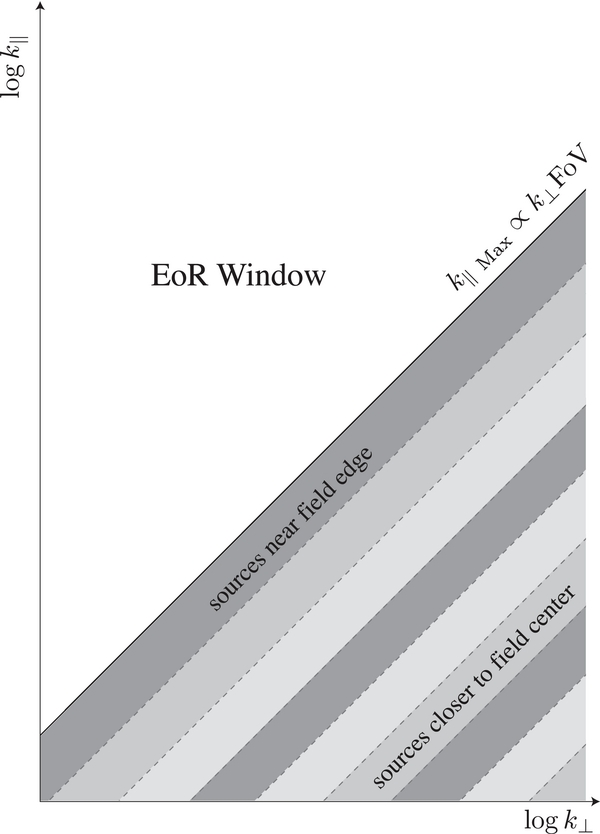
\includegraphics[width=0.49\textwidth]{figures/chapter1/morales-foreground-wedge-illustration} &
        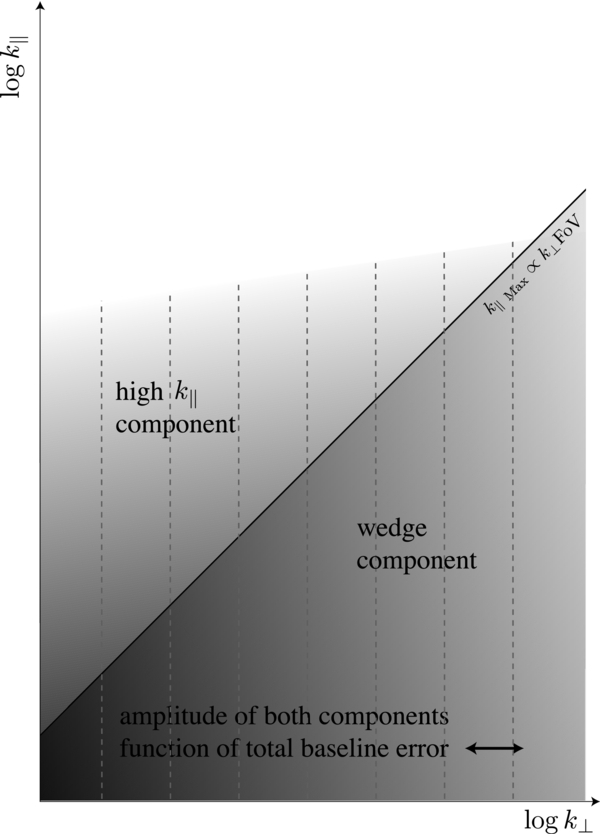
\includegraphics[width=0.49\textwidth]{figures/chapter1/morales-foreground-wedge-calibration-errors} \\
        (a) & (b) \\
    \end{tabular}
    \caption{
        (a) Illustration of the foreground wedge. The emission near the edge of the foreground wedge
        typically originates from sources located far from the delay center.
        (b) Illustration of the contamination arising after calibration errors. Emission leaks out
        of the foreground wedge and into the otherwise clean ``EoR Window.''
        Reproduced from \citet{2012ApJ...752..137M} (permission not yet received).
    }
    \label{fig:morales-foreground-wedge}
\end{figure*}

\subsection{Foreground Avoidance}

In the absence of a reliable foreground model, some power spectrum experiments---notably
PAPER---have opted for a delay-spectrum technique to separate foreground emission from the
cosmological 21\,cm signal \citep{2012ApJ...756..165P}. This technique has also been coined
``foreground avoidance,'' because it applies a transformation to the dataset that---under ideal
circumstances---restricts the extent of foreground contamination to a wedge-like feature in power
spectrum space (see Figure~\ref{fig:morales-foreground-wedge} for an illustration). The existence of
the foreground wedge can be seen with a simple argument presented below.

In the flat-sky approximation, an interferometer measures a visibility $V^{ij}_\nu$ between the
pair of antennas $i$ and $j$ at the frequency $\nu$. For isotropic antennas, the visibility is
related to the sky brightness $I_\nu(l, m)$ through
\begin{equation}\label{eq:flat-sky-visibilities}
    V^{ij}_\nu = \int I_\nu(l, m)\,\exp\Big(2\pi i (ul + vm)\Big)\,\d l\,\d m\,,
\end{equation}
where $l$ and $m$ are direction cosines, and $u$ and $v$ are the east--west and north--south
components of the baseline vector measured in units of wavelengths.
Equation~\ref{eq:flat-sky-visibilities} is a Fourier transform over the plane of the sky, and so in
order to construct a three-dimensional power spectrum, an additional Fourier transform along the
line of sight is needed. This can be accomplished by expanding the comoving distance with the Taylor
expansion $r \approx r_0 + (\partial r/\partial \nu)(\nu - \nu_0)$ at the appropriate redshift.
Under this approximation, a Fourier transform along the line of sight is a Fourier transform over
frequency.  The Fourier dual variable to the frequency is delay. That is, by taking a Fourier
transform along the line of sight, we are actually undoing the F stage of the correlator, and
computing a series of correlations at a range of time delays.  Consequently, the perpendicular
wavenumber $k_\perp \propto \text{the baseline length}$, and the parallel wavenumber $k_\parallel
\propto \text{delay}$.

For a smooth spectrum radio source, the maximum possible delay between the two antennas $i$ and $j$
is the light-travel time between the two antennas. More generally the delay is given by the path
difference, and sources located far from the delay center have larger delays. The pattern of
contamination for smooth spectrum radio sources is therefore generally restricted to a wedge-like
structure that is illustrated in the left panel of Figure~\ref{fig:morales-foreground-wedge}.  With
the foreground emission contained within this wedge, the power spectrum may simply be estimated from
the set of modes outside of the wedge, and in this way avoid the contamination of the foreground
emission.

The technique of foreground avoidance is predicated on the assumption that the spectral structure of
the foreground emission is smooth enough for it to be contained within the foreground wedge.
Instrumental chromaticity and polarization leakage are of particular concern. Faraday-rotated
linearly polarized emission, for instance, is not contained within the foreground wedge.
Furthermore, widefield effects such as baseline foreshortening towards the horizon can introduce
additional leakage \citep{2015ApJ...804...14T}.

\subsection{Foreground Subtraction}

A more direct approach to suppressing foreground contamination is to model and remove as much of the
contamination as possible. This has been the focus of the LOFAR EoR KSP, which has dedicated
substantial resources towards subtracting all of the radio emission in their deep fields
\citep{2017ApJ...838...65P}. In total within a 3$\arcdeg$ field of view, they have removed almost
21,000 sky components down to a limit of 3\,mJy using over 100 direction-dependent calibrations to
account for beam and ionospheric errors.

On top of this modeling effort, \citet{2017ApJ...838...65P} applied Generalized Morphological
Component Analysis \citep[GMCA;][]{2013MNRAS.429..165C} to suppress the residual contamination.
GMCA is a blind technique for decomposing the remaining emission into a number of statistically
independent components. In fact, the implementation used here did not incorporate any prior
astrophysical information about the nature of the foreground emission, which raises the possibility
of subtracting the cosmological 21\,cm emission alongside the foreground emission.
\citet{2013MNRAS.429..165C} showed that they could recover the 21\,cm signal for simulated LOFAR
data with signal loss between 10--40\%, but real instrumental considerations could drive the signal
loss higher. Future iterations of this technique will likely need to build in some prior
astrophysical information.

Unanticipated signal loss is not a new problem to foreground subtraction efforts.
\citet{2013MNRAS.433..639P} used detailed simulations to compute the signal loss when removing
foreground emission using a Singular Value Decomposition (SVD), which is another blind technique for
subtracting foreground emission. Similarly \citet{2016MNRAS.463.4317P} realized that their process
for removing point sources with a direction-dependent calibration was also capable of
unintentionally removing diffuse foreground emission. Finally, Cheng et al. (in prep.) discovered
that using a covariance matrix derived from the measured data can lead to signal loss due to the
down-weighting of the cosmological 21\,cm signal.

\subsection{Instrumental Calibration}

The process of avoiding or subtracting foreground emission is compounded by the difficulty of
calibrating low-frequency interferometers.  With a field of view typically $\gtrsim10\arcdeg$ across
and a proclivity for the most troublesome sources to be far from the delay center (see
Figure~\ref{fig:morales-foreground-wedge}), a detailed understanding of the---potentially
inhomogeneous---antenna response pattern is essential.  For instance, \citet{2015PhRvD..91h3514S}
concluded that the Canadian Hydrogen Intensity Mapping Experiment (CHIME) must measure its beam to
better than one part in $10^{-4}$ to avoid biasing a measurement of the power spectrum.
Furthermore, a standard sky-based calibration procedure will require a model for the entire field of
view. An incomplete sky model will introduce ripples into the bandpass that impedes the observer's
ability to separate foreground emission from the cosmological 21\,cm emission \citep[e.g.,
Figure~\ref{fig:morales-foreground-wedge};][]{2016MNRAS.461.3135B, 2017MNRAS.470.1849E}.

In order to address some of the difficulties associated with sky-based calibration, some power
spectrum experiments---notably PAPER and HERA---have implemented redundant baseline calibration
\citep{2010MNRAS.408.1029L}. While redundant calibration is useful for discovering instrumental
errors and deriving calibration parameters in a way that is robust to modeling errors, there are
some calibration parameters that cannot be constrained with redundant calibration.  Notably this
includes the overall bandpass, which must still be measured from the spectrum of a known point
source. Yet at this time, few flux calibrators exist at frequencies below 200\,MHz
\citep{2012MNRAS.423L..30S, 2017ApJS..230....7P}.

Propagation effects through the ionosphere additionally complicate low-frequency observations. The
refractive index of the ionosphere $n = \sqrt{1 - \nu_\text{plasma}^2/\nu^2}$, where the plasma
frequency $\nu_\text{plasma}$ is typically $\sim10\,\text{MHz}$. When the diffractive scale of the
ionosphere is small, point sources can break apart into multiple images \citep{2015MNRAS.453..925V},
but even when ionospheric conditions are mild, it can still contribute 50\% amplitude scintillation
on 13\,s timescales and 20$\arcmin$ variable refractive offsets on 10\,minute timescales (see
\S\ref{sec:ionosphere-conditions}).  At least while conditions are mild, ionospheric propagation
effects may be described with a direction-dependent calibration. However, as previously discussed,
direction-dependent calibration may lead to unintentional signal loss, and must therefore be applied
judiciously.

\section{Future Outlook}\label{sec:intro-future-outlook}

\begin{figure}[t]
    \centering
    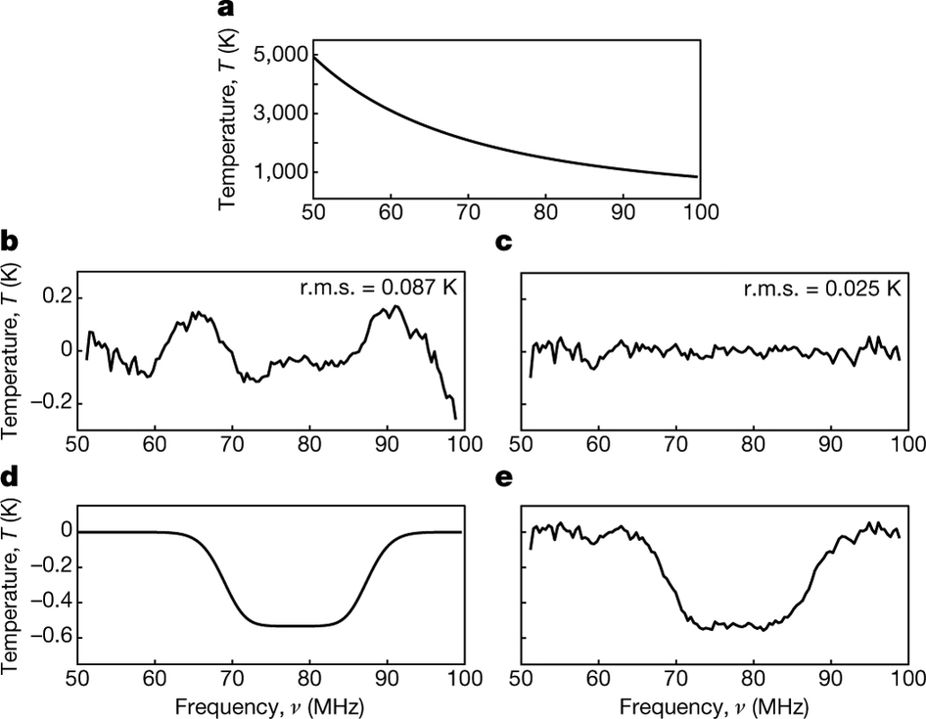
\includegraphics[width=\textwidth]{figures/chapter1/bowman-2018-absorption-trough}
    \caption{
        (a) The calibrated sky spectrum measured by the EDGES experiment.
        (b) The residuals after fitting a model of the foreground emission.
        (c) The residuals after performing a joint fit of the foreground emission and an absorption
        trough.
        (d) The best-fit absorption trough.
        (e) The best-fit absorption trough including residual noise.
        This figure is reproduced with permission from \citet{2018Natur.555...67B}.
    }
    \label{fig:bowman-absorption-trough}
\end{figure}

Despite the practical difficulties involved in detecting the 21\,cm transition from the EoR and
Cosmic Dawn, it promises to open up a new window towards the high-redshift universe and the first
generation of stars and galaxies.  Recently, a significant development came from the first putative
detection of the Cosmic Dawn through the global 21\,cm signal by the EDGES experiment
\citep{2018Natur.555...67B}. In this paper, the authors claimed the detection of an absorption
feature centered at $78\,\text{MHz}$ ($z\sim17$), which they attribute to early star formation and
heating (see Figure~\ref{fig:bowman-absorption-trough}).

The absorption feature reported by \citet{2018Natur.555...67B} is remarkable for its extreme
amplitude ($\sim 500\,\text{mK}$), which cannot be attained through purely adiabatic cooling of the
IGM.  Currently there is some skepticism in regards to how EDGES modeled and subtracted foreground
emission \citep{2018arXiv180501421H}, but the result has nevertheless sparked a flurry of new ideas
ranging from the absurd (i.e., $\Omega_m = \Omega_b$) to the exotic.  The most plausible of these
theories are new ideas for either cooling the IGM \citep[e.g.,][]{2018Natur.555...71B} or positing a
new source of radio emission originating from $z > 20$ \citep[e.g.,][]{2018arXiv180301815E}.

As an example, \citet{2018Natur.555...71B} noted that because Compton scattering of CMB photons off
of residual free electrons after recombination heats the baryons until $z\sim 150$, the dark matter
has been able to cool adiabatically for longer and therefore has a lower temperature. A potential
interaction between baryons and dark matter could therefore allow the baryons to cool
super-adiabatically. In this scenario, the amplitude of the 21\,cm power spectrum at $z\sim 17$ is
expected to be $\sim (140\,\text{mK})^2$, substantially larger than previous predictions.  In a
separate paper, \citet{2018arXiv180303091B} also argued that existing dark matter experiments make
this possibility somewhat unlikely, which is a reflection of the fact that this initial detection
has produced more questions than answers.

Power spectrum experiments can offer an independent verification and continue to advance in
sophistication and sensitivity with upgrades to LOFAR, the MWA, and the construction of the Hydrogen
Epoch of Reionization Array \citep[HERA;][]{2017PASP..129d5001D}. HERA will be composed of $\sim350$
parabolic dishes (each 14\,m in diameter) hexagonally packed within a core 300\,m across.  Each dish
will be equipped with a feed that operates between 50 and 250\,MHz ($z\sim5-27$). HERA incorporates
lessons learned from the preceding PAPER experiment, and so with a major increase in collecting area
with respect to PAPER, promises to deliver a compelling detection of the 21\,cm power spectrum.
On even longer timescales, the SKA may be capable of constructing a tomographic map of the universe
through the 21\,cm transition \citep{2013ExA....36..235M}.

At Caltech, multiple experiments are attempting to measure spectral features from the EoR and Cosmic
Dawn. The Owens Valley Radio Observatory Long Wavelength Array (OVRO-LWA) is a 288 element
interferometer with instantaneous bandwidth covering 30--85\,MHz. In this thesis I will present, to
date, the highest angular-resolution maps of the sky available below 100\,MHz using the OVRO-LWA and
a new imaging technique designed for drift-scanning interferometers. These maps have been made
publicly available on the Legacy Archive for Microwave Background Data Analysis (LAMBDA).\footnote{
    \url{https://lambda.gsfc.nasa.gov/}
}
I will also present the deepest upper limits on the amplitude of the 21\,cm power spectrum of the
Cosmic Dawn, and the only existing limits at $z > 18$. Figure~\ref{fig:history-of-the-universe}
presents a radial map of the universe that compares the comoving radial distances probed by the
OVRO-LWA and HERA to other probes of the high-redshift universe.

\begin{figure}[t]
    \centering
    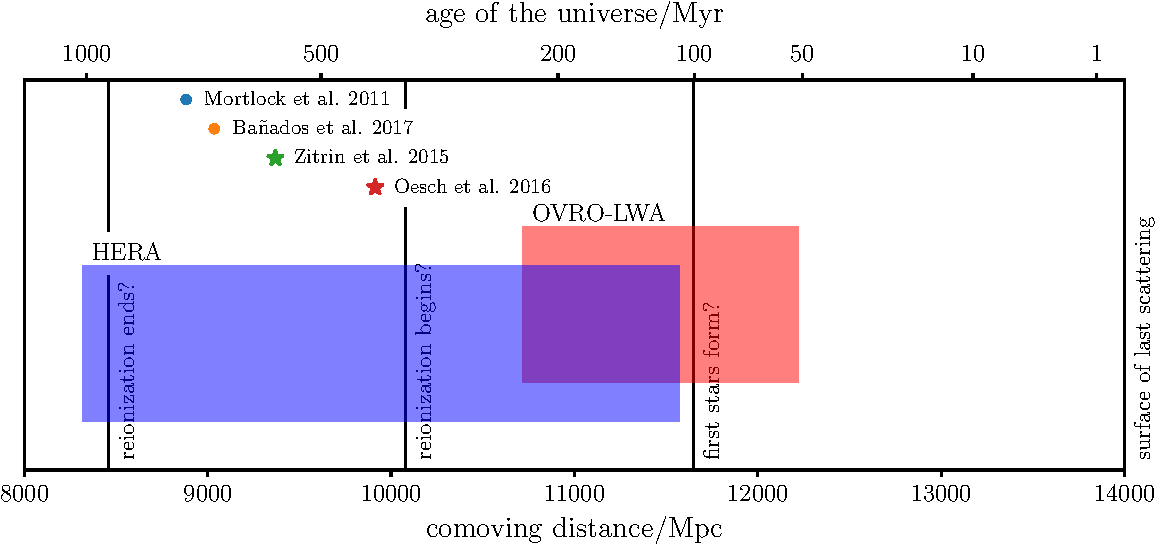
\includegraphics[width=\textwidth]{figures/chapter1/history-of-the-universe/history-of-the-universe}
    \caption{
        A radial map of the universe. Known quasars are marked with circles and galaxies are marked
        with stars. The range of comoving distances probed by the OVRO-LWA and HERA are marked with
        a red rectangle and a blue rectangle respectively.
    }
    \label{fig:history-of-the-universe}
\end{figure}

These measurements are highly complementary to other ongoing experiments at Caltech, notably the CO
Mapping Array Pathfinder \citep[COMAP;][]{2016AAS...22742606C} and the Tomographic Ionized carbon
Intensity Mapping Experiment Pilot \citep[TIME-Pilot;][]{2017AAS...22912501C}, which aim to
ultimately detect transitions of CO and \ion{C}{2} from the EoR respectively. While the 21\,cm power
spectrum of the EoR originates from the neutral gas surrounding the expanding ionized bubbles, CO
and \ion{C}{2} emission originates from the sites of star formation, therefore helping to build a
more complete picture of the EoR.  Furthermore, correlations with the 21\,cm signal will help to
mitigate systematics in both measurements.

In Chapter~\ref{chapter2} I will introduce the OVRO-LWA, its construction, commissioning, and the
its calibration. In Chapter~\ref{chapter3} I will describe Tikhonov-regularized $m$-mode analysis
imaging and cleaning, and demonstrate its application by generating maps of the full sky visible
from OVRO with $15\arcmin$ angular resolution. In Chapter~\ref{chapter4} I will present the most
sensitive upper limits on the 21\,cm power spectrum of the Cosmic Dawn using a new technique for
foreground filtering, and finally in Chapter~\ref{chapter5} I will present my conclusions.

\myputbib{thesis}
\end{bibunit}

